% D.7 角平分线 + 距离相等：AD 平分∠BAC，DE⊥AB 于 E，DF⊥AC 于 F
\documentclass[tikz,border=4pt]{standalone}
\usepackage{ctex}
\usepackage{amsmath}
\usetikzlibrary{calc}
\begin{document}
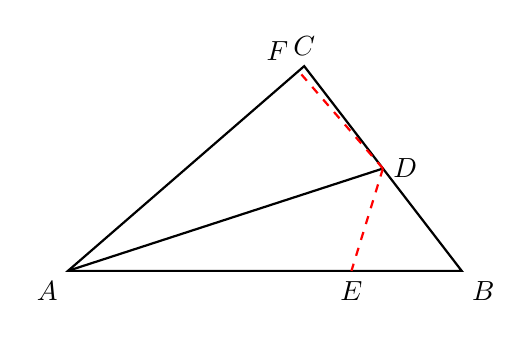
\begin{tikzpicture}[scale=1.0, thick]
  \coordinate (A) at (0, 0);
  \coordinate (B) at (5, 0);
  \coordinate (C) at (3, 2.6);
  \coordinate (D) at ($(B)!0.5!(C)$);
  % E = D 在 AB 上的投影
  \coordinate (E) at (3.6, 0);
  % F = D 在 AC 上的投影；AC 方向 (3,2.6)/|.|
  \pgfmathsetmacro{\ax}{3} \pgfmathsetmacro{\ay}{2.6}
  \pgfmathsetmacro{\an}{sqrt(\ax*\ax+\ay*\ay)}
  \pgfmathsetmacro{\dt}{(4*\ax + 1.3*\ay)/(\ax*\ax+\ay*\ay)}
  \coordinate (F) at ({\dt*\ax}, {\dt*\ay});

  \draw (A) -- (B) -- (C) -- cycle;
  \draw (A) -- (D);
  \draw[red, dashed] (D) -- (E);
  \draw[red, dashed] (D) -- (F);

  \node[below left]  at (A) {$A$};
  \node[below right] at (B) {$B$};
  \node[above]       at (C) {$C$};
  \node[right]       at (D) {$D$};
  \node[below]       at (E) {$E$};
  \node[above left]  at (F) {$F$};
\end{tikzpicture}
\end{document}
